\subsection{Scalar model with mixing (SMM)} \label{sub:SMM} 
%%%%%%%%%%%%%%%%%%%%%%%%%%%%%%%%%%%%%%%%%%%%%%%%%%%%%%%%%%%%%%
We consider a simple extension to the scalar-mediated models previously recommended by the ATLAS/CMS Dark Matter Forum (DMF,~\cite{Abercrombie:2015wmb}).  With respect to those models, the scalar model with mixing (SMM, recently explored in Ref.~\cite{Bauer:2016gys}) includes a new scalar (s) that couples only to DM fermions ($\chi$) and to the SM Higgs doublet (h): 

\begin{equation} \label{eq:Linteractions}
{\cal L} \supset -y_{\rm DM} \hspace{0.25mm} s \hspace{0.25mm} \bar \chi \chi  - \mu \hspace{0.25mm} s \hspace{0.25mm} |h|^2 \, 
\end{equation}

where $y_{\rm DM}$ is a dark-sector Yukawa coupling. The trilinear portal interaction (\textcolor{red}{KH: eqn is missing the new term for mono-H}) leads to h-s mixing, which is parameterized by the angle $\theta$:  

\begin{equation} \label{eq:mixing}
\begin{pmatrix} h_1 \\[2mm] h_2 \end{pmatrix} = \begin{pmatrix} \cos \theta & \hspace{1mm}   \sin \theta \\[2mm] -\sin \theta & \hspace{1mm} \cos \theta \end{pmatrix} \begin{pmatrix} h \\[2mm] s \end{pmatrix},
\end{equation}

We consider the h1 mass eigenstate to be the observed 125 GeV Higgs-like boson.  The h2 state is the analogue of the new scalar mediator in the DMF model.  As a result of mixing, the h1 and h2 eigenstates both obtain couplings to SM and DM fermions.  In particular, and in contrast with the earlier DMF models, the h2 mediator now also obtains couplings to the electroweak vector bosons.  The h2 fermionic couplings in the SMM correspond to those in the earlier DMF scalar models with the following replacements:    

\begin{equation} \label{eq:replacements}
g_{\rm DM} \rightarrow cos\theta, g_{\rm SM} \rightarrow -sin\theta ~\\
\end{equation}

The SMM effectively introduces one additional model parameter relative to the set of masses and couplings considered in the DMF.  The full list of model parameters are as follows: 

\begin{itemize}
\item $m_{\chi}$ : the mass of the DM fermion
\item $m_{h2}$ : the mass of the new scalar mediator
\item $y_{DM}$ : the Yukawa coupling strength to the DM fermion
\item $\theta$ : the h-s mixing angle (conventionally, $\sin\theta$ )
\item $g_{b}$ : the coupling strength for ... 
\end{itemize}

In general, DM production rates and kinematics in the SMM differ from those of the scalar-mediated DMF models.  For example, when Higgs boson decays to DM are kinematically allowed, the Higgs serves as the primary DM mediator.  Likewise, Higgs decays to DM are prohibited when $2m_{\chi} > m_{h1}$; a sufficiently heavy h2 will function as the DM mediator in this case.  Figures~\ref{fig:SMMkinematics} and~\ref{fig:SMMrates} compare the $\t\bar{t} + \chi\bar{\chi}$ kinematics and production rates expected for these two scenarios.

%--------------------------------
\begin{figure}[hbtp]
\centering
\begin{subfigure}[b]{0.49\textwidth}
  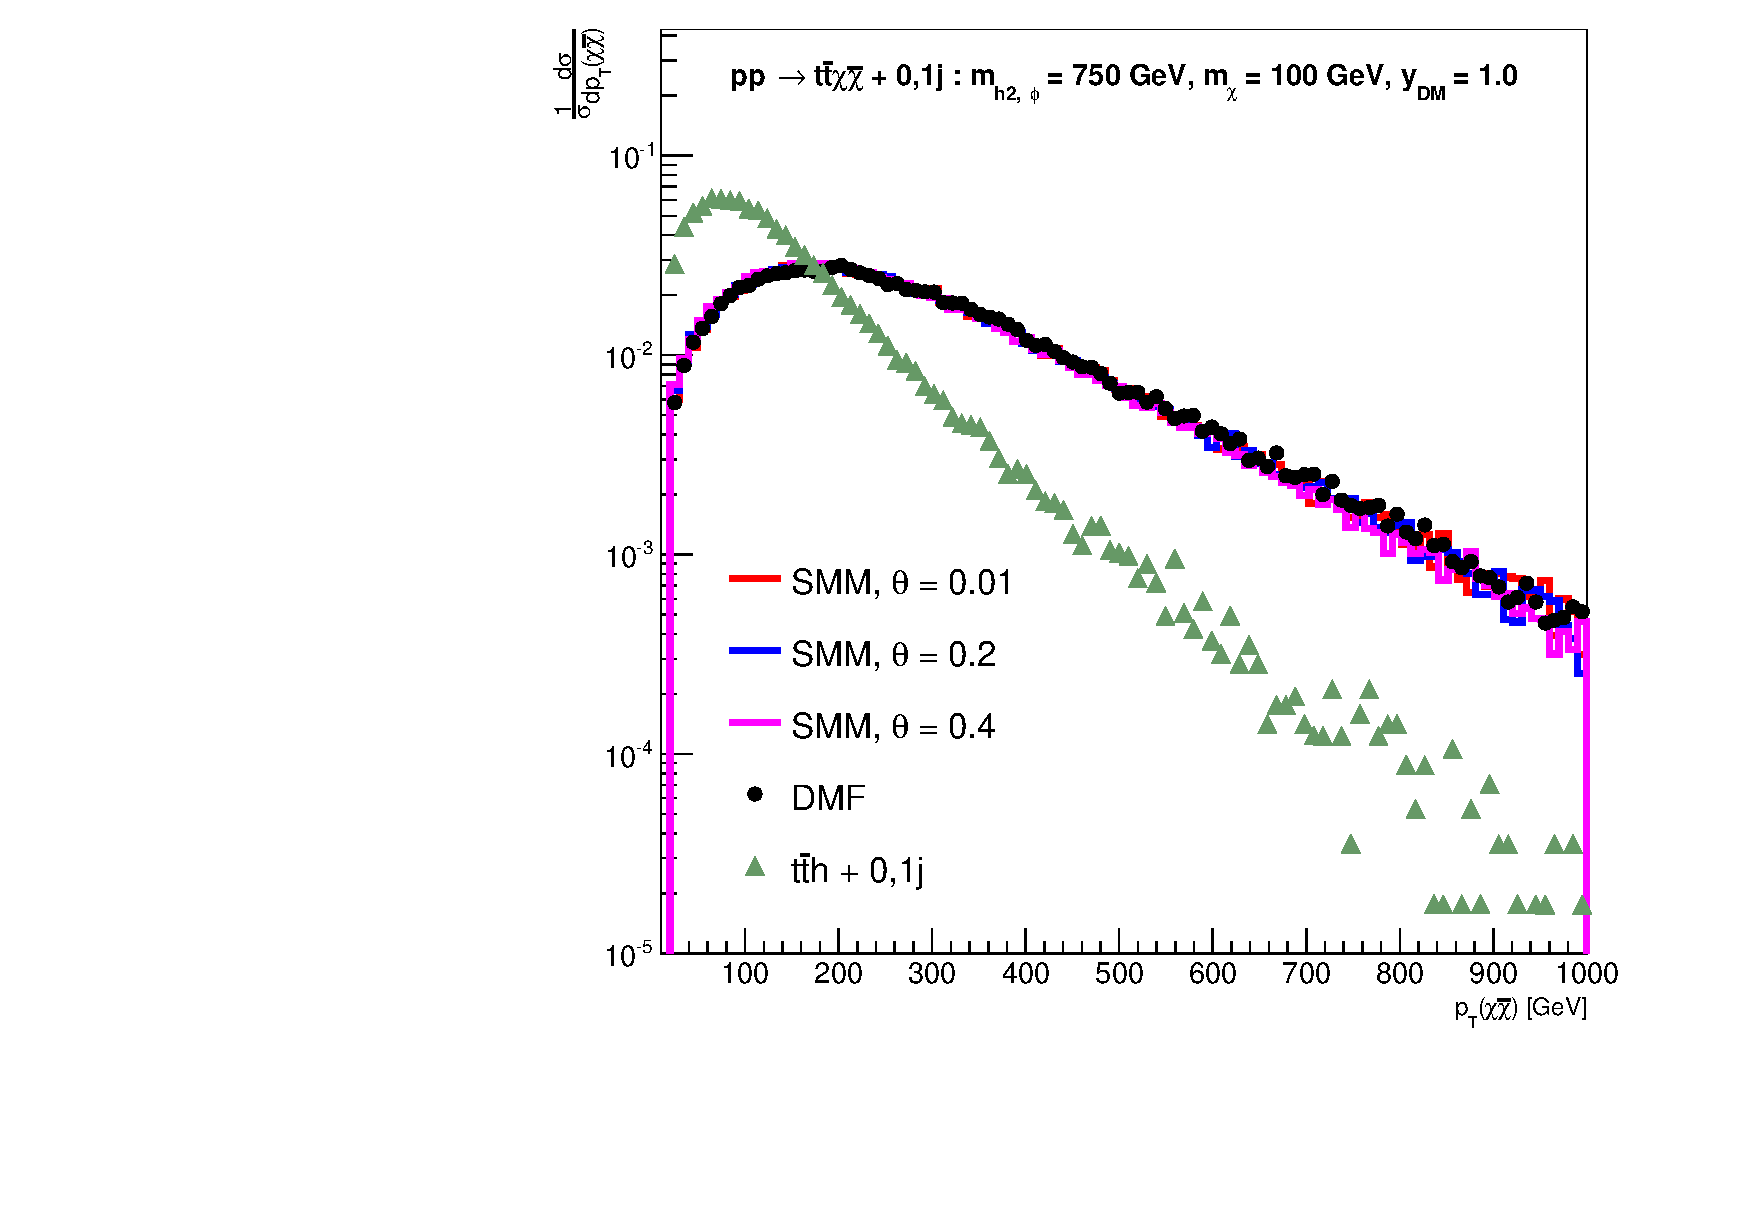
\includegraphics[width=\textwidth]{{./figures/ttDM_kinematics_MMed_750_mDM_100_gDM_1.0_vs_DMF}.pdf}
\end{subfigure}
\begin{subfigure}[b]{0.49\textwidth}
  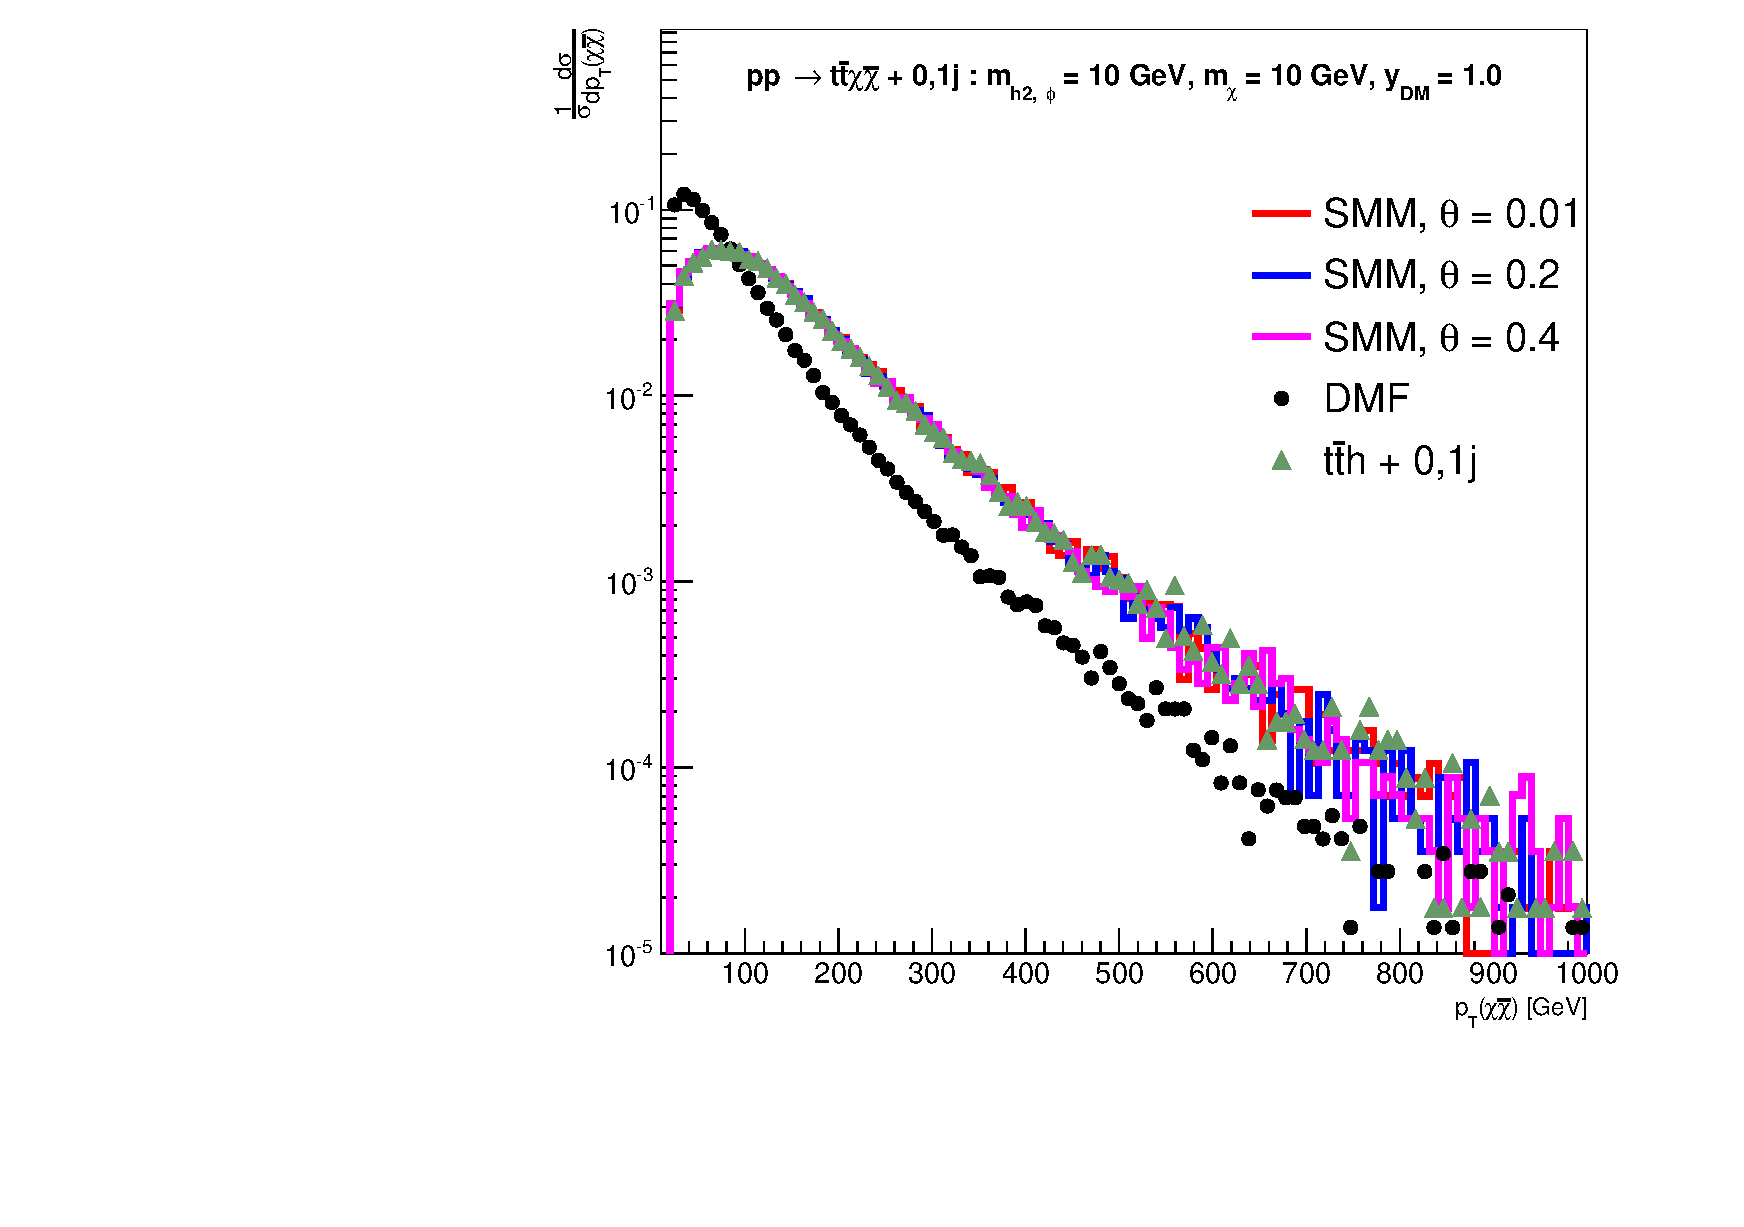
\includegraphics[width=\textwidth]{{./figures/ttDM_kinematics_MMed_10_mDM_10_gDM_1.0_vs_DMF}.pdf}

\end{subfigure}
~\\
  \caption{ Blah ... }
  \label{fig:SMMkinematics}
\end{figure}
%--------------------------------
\begin{figure}[hbtp]
\centering
\begin{subfigure}[b]{0.49\textwidth}
  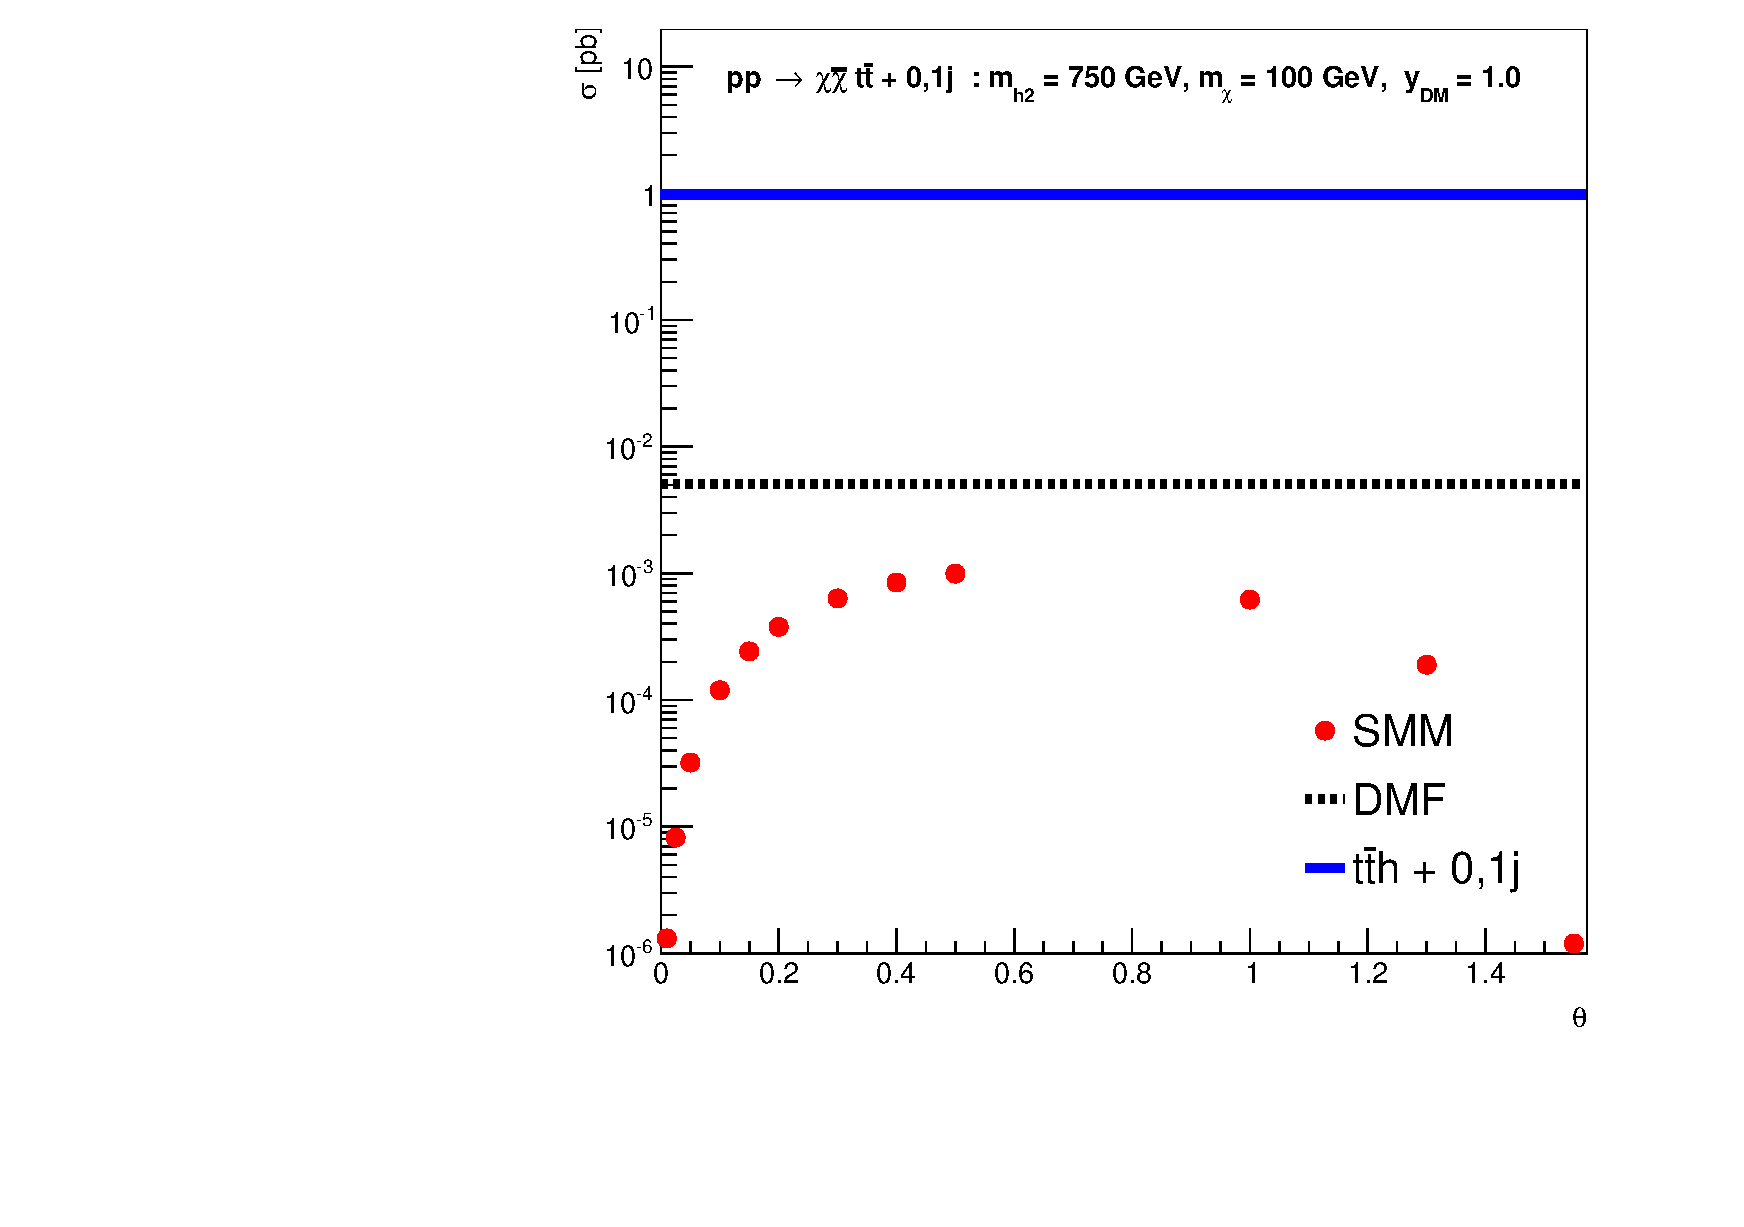
\includegraphics[width=\textwidth]{{./figures/ttDM_xsec_vs_theta_mDM_100_mMed_750_g_1.0}.pdf}
\end{subfigure}
\begin{subfigure}[b]{0.49\textwidth}
  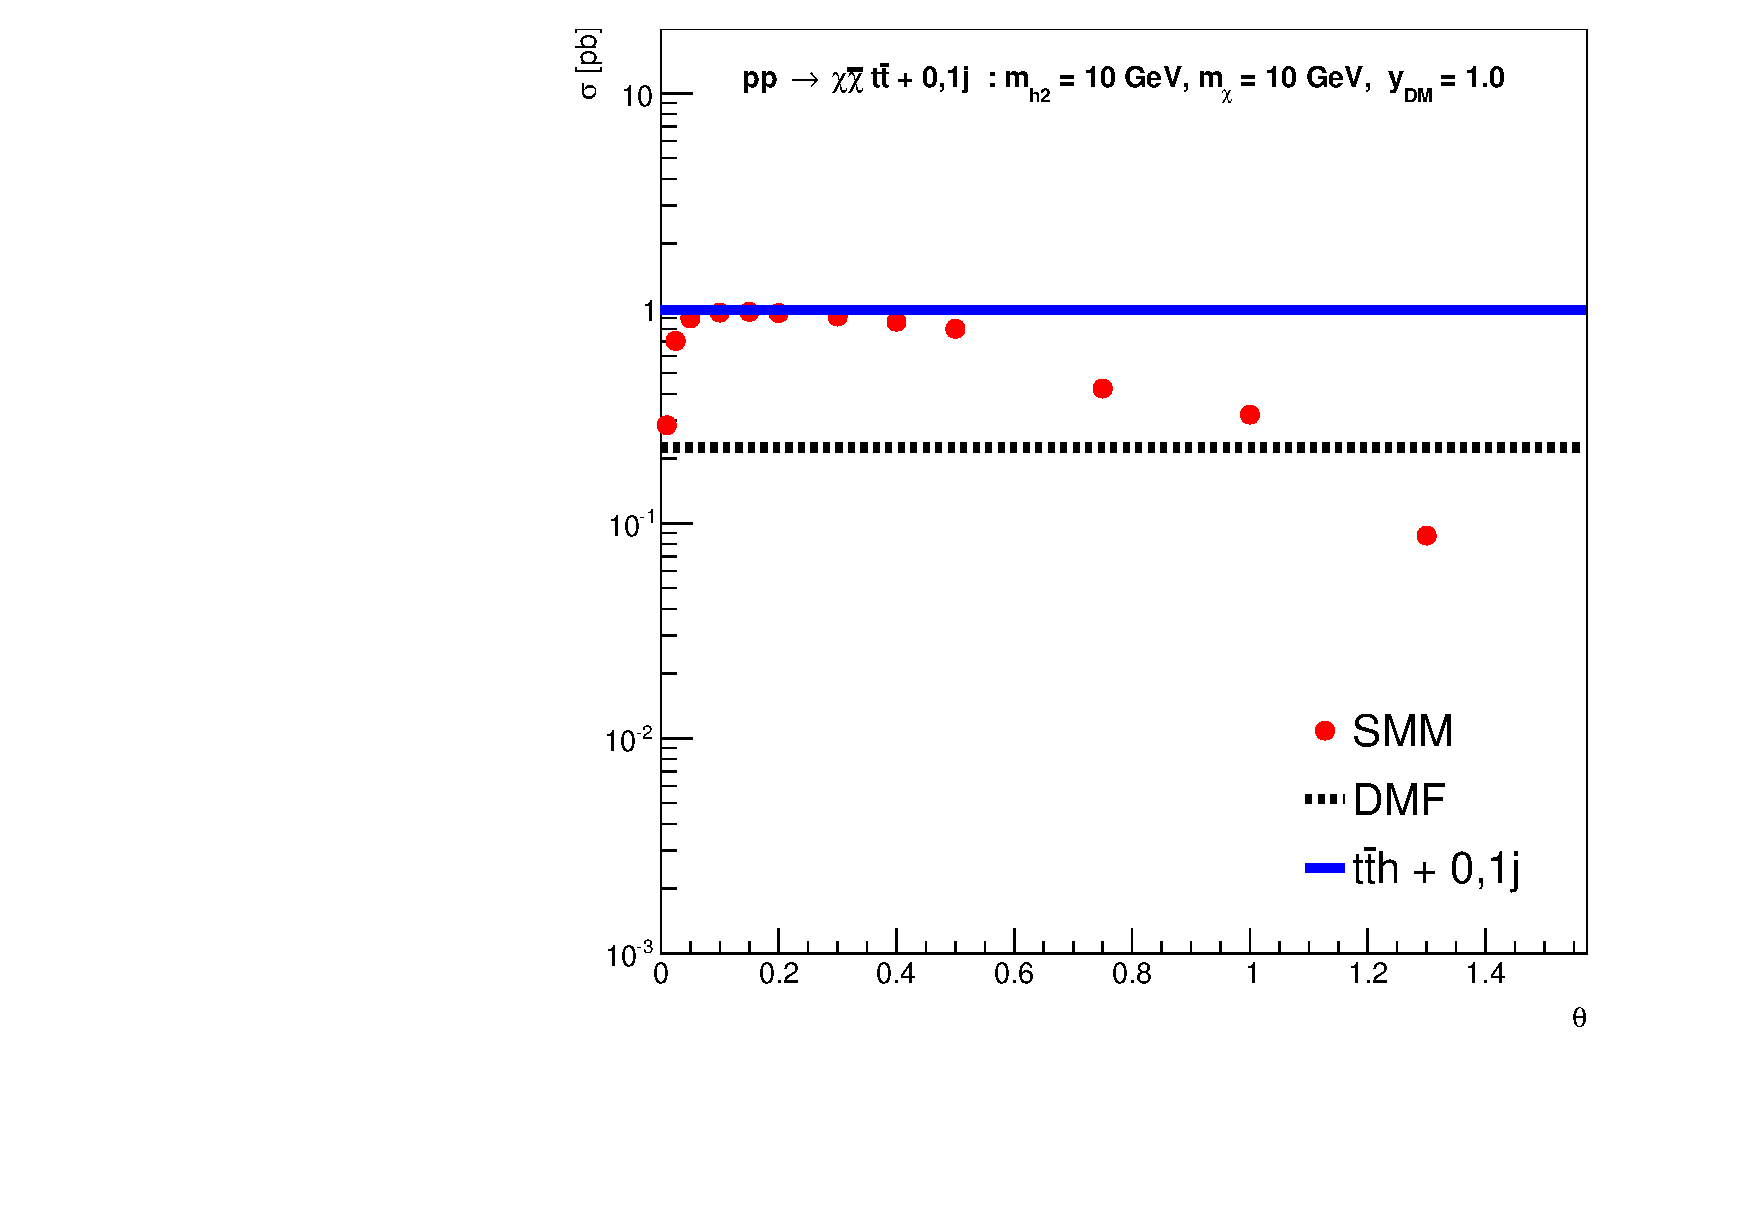
\includegraphics[width=\textwidth]{{./figures/ttDM_xsec_vs_theta_mDM_10_mMed_10_g_1.0}.pdf}
\end{subfigure}
~\\
  \caption{ Blah ... }
  \label{fig:SMMrates}
\end{figure}
%--------------------------------

Mixing between the new scalar and the SM Higgs introduces additional constraints on the SMM relative to the DMF scalar model.  Global fits~\cite{Farzinnia:2013pga,Belanger:2013kya} to LHC Run 1 data find $sin\theta \lesssim 0.4$, which implies that the state h1 (h2) is mostly Higgs-like (singlet-like). Constraints on $\theta$ also arise from the oblique parameters T and S~\cite{Baek:2011aa}, but are weaker than those that follow from the Higgs boson measurements.  LHC searches for invisible Higgs decays can also impose significant constraints on SMM parameters.  For example, Figure~\ref{fig:recast} shows the projected luminosity required to achieve the indicated bounds on $sin\theta$ and $y_{\rm DM}$ from a recasting of the results of Ref.~\cite{CMShinv}.

%--------------------------------
\begin{figure}[hbtp]
\centering
\begin{subfigure}[b]{0.49\textwidth}
  
\includegraphics[width=\textwidth]{./figures/placeholder.jpg}
\end{subfigure}
\begin{subfigure}[b]{0.49\textwidth}
  
\includegraphics[width=\textwidth]{./figures/placeholder.jpg}
\end{subfigure}
~\\
  \caption{ Blah ... }
  \label{fig:recast}
\end{figure}
%--------------------------------

Based on these considerations, we recommend that the following SMM benchmark scenarios be explored: 
~\\
...




